\pdfminorversion=7
\documentclass[10pt]{article}
\usepackage[margin=0.85in]{geometry}
\usepackage[T1]{fontenc}
\usepackage[utf8]{inputenc}
\usepackage{lmodern}
\usepackage{amsmath,amssymb,amsthm}
\usepackage{booktabs}
\usepackage{tabularx}
\usepackage{enumitem}
\usepackage{xcolor}
\usepackage{listings}
\usepackage{graphicx}
\usepackage{tikz}
\definecolor{bpgreen}{HTML}{1CAC78}
\definecolor{bpdef}{HTML}{B0ECA3}
\definecolor{bpblue}{HTML}{1F5FD6}
\usetikzlibrary{arrows.meta,positioning,shapes.geometric}
\usepackage[colorlinks=true,linkcolor=blue!50!black,citecolor=blue!50!black,urlcolor=blue!50!black]{hyperref}

\graphicspath{{./}{report/}}

\setlist{itemsep=1.5pt,topsep=3pt}
\emergencystretch=3em
\let\origus\_
\renewcommand{\_}{\origus\allowbreak}

\newtheorem{theorem}{Theorem}
\newcommand{\C}{\mathbb{C}}
\newcommand{\R}{\mathbb{R}}
\newcommand{\Z}{\mathbb{Z}}
\newcommand{\N}{\mathbb{N}}
\newcommand{\Quat}{\mathbb{H}}
\newcommand{\Oct}{\mathbb{O}}
\newcommand{\Kfield}{\mathbb{K}}
\newcommand{\Hyp}{\mathbf{H}}
\newcommand{\Tr}{\operatorname{Tr}}
\newcommand{\Vol}{\operatorname{Vol}}
\newcommand{\Hess}{\operatorname{Hess}}
\newcommand{\code}[1]{\texttt{#1}}
\providecommand{\llbracket}{[\![}
\providecommand{\rrbracket}{]\!]}

% ---- Auto-populated Repository & Audit Metrics ----
\newcommand{\LeanToolchain}{leanprover/lean4:v4.35.0}
\newcommand{\NModules}{12}
\newcommand{\NLines}{5{,}247}
\newcommand{\NTotalNodes}{27}
\newcommand{\NProvedNodes}{19}
\newcommand{\NDefNodes}{8}
\newcommand{\NLeanDecls}{227}
\newcommand{\NSorryAx}{0}

\lstdefinelanguage{lean}{
  morekeywords={theorem,lemma,def,structure,class,where,by,fun,let,have,exact,obtain,refine,import,namespace,end,variable,open,Nonempty,Fintype},
  sensitive=true, morecomment=[l]{--}, morecomment=[s]{/-}{-/}, morestring=[b]"}
\lstset{language=lean,basicstyle=\ttfamily\scriptsize,keywordstyle=\bfseries\color{blue!50!black},
  commentstyle=\itshape\color{gray},columns=fullflexible,keepspaces=true,frame=single,framerule=0.3pt,
  xleftmargin=4pt,xrightmargin=4pt,breaklines=true,
  literate={→}{{$\to$}}1 {∀}{{$\forall$}}1 {∃}{{$\exists$}}1 {¬}{{$\neg$}}1 {≤}{{$\le$}}1 {ℕ}{{$\mathbb{N}$}}1
           {ℝ}{{$\mathbb{R}$}}1 {ℤ}{{$\mathbb{Z}$}}1 {ℂ}{{$\mathbb{C}$}}1 {⟨}{{$\langle$}}1 {⟩}{{$\rangle$}}1
           {⌊}{{$\lfloor$}}1 {⌋}{{$\rfloor$}}1 {σ}{{$\sigma$}}1 {ε}{{$\varepsilon$}}1 {ϕ}{{$\phi$}}1
           {∧}{{$\wedge$}}1 {∘}{{$\circ$}}1 {₁}{{$_1$}}1 {₂}{{$_2$}}1 {₃}{{$_3$}}1 {₀}{{$_0$}}1
           {·}{{$\cdot$}}1 {∨}{{$\vee$}}1 {⊤}{{$\top$}}1 {<}{{$<$}}1 {‖}{{$\|$}}1 {•}{{$\bullet$}}1
           {∑}{{$\sum$}}1 {∏}{{$\prod$}}1 {∈}{{$\in$}}1 {∂}{{$\partial$}}1 {∫}{{$\int$}}1 {ₗ}{{$_l$}}1
           {α}{{$\alpha$}}1 {ξ}{{$\xi$}}1 {μ}{{$\mu$}}1 {π}{{$\pi$}}1 {λ}{{$\lambda$}}1}

\title{\vspace{-1.8em}\textbf{Machine-Checked Formalization of the Besson--Courtois--Gallot\\Barycenter Method and Ruan's Octonionic Repair in Lean~4}}
\author{Pablo Su\'arez-Serrato}
\date{November 2026\vspace{-1.0em}}

\begin{document}
\maketitle

\begin{abstract}
\noindent
We present the executive audit and architectural synthesis of the core Lean~4
(\code{\LeanToolchain}) library \code{BCG} inside \code{formalized-barycenter-methods}, formalizing
the Besson--Courtois--Gallot \cite{BCG95} and Souto \cite{Sou08} barycenter method across real
hyperbolic spaces $\R\Hyp^n$, associative rank-one symmetric spaces $\Kfield\Hyp^m$
($\Kfield \in \{\R, \C, \Quat\}$), and Yuping Ruan's 2024 repair \cite{Rua24} of the
long-standing octonionic gap on the $16$-dimensional Cayley hyperbolic plane $\Oct\Hyp^2$.
Across \NModules{} library modules (\NLines{} lines of Lean~4 code), \NTotalNodes{} \code{leanblueprint} nodes,
and \NLeanDecls{} tracked blueprint declarations, the entire core library compiles with \textbf{\NSorryAx{}
\code{sorryAx}} and depends exclusively on Lean's three standard axioms (\code{propext},
\code{Classical.choice}, \code{Quot.sound}). All \NTotalNodes{} nodes of the \code{leanblueprint}
dependency graph are green (\NProvedNodes{} proved theorem nodes in dark green \code{\#1CAC78} and
\NDefNodes{} definition nodes in green \code{\#B0ECA3}). Downstream non-smooth extensions and
geometric applications reside in the companion subrepositories
\code{rcd-entropy-degree-rigidity} and \code{alexandrov-entropy-degree-applications}.
\end{abstract}

\section{Executive Audit Verdict and Verification Gate}

The formalization of the Besson--Courtois--Gallot volume-entropy and rigidity theorems, together with
Ruan's perturbed log-concavity repair for $\Oct\Hyp^2$, has passed an automated end-to-end kernel and
blueprint audit executed via \code{verify\_blueprint.py} and \code{report\_tool.py}. No custom
\code{axiom}, \code{sorry}, \code{admit}, \code{unsafe}, or \code{implemented\_by} occurs anywhere in the
codebase.

\begin{table}[!ht]
\centering\footnotesize
\renewcommand{\arraystretch}{1.12}
\begin{tabularx}{\textwidth}{@{}>{\bfseries}l l X r@{}}
\toprule
Audit Gate Component & Tool / Target & Verification Scope & Result \\
\midrule
Full Library Compilation & \code{lake build} & \NModules{} library modules (\NLines{} LOC, \code{\LeanToolchain}) & \textbf{Pass} (0 errors) \\
Axiom \& Soundness Census & \code{\#print axioms} & All \NLeanDecls{} declarations in \code{blueprint/lean\_decls} & \textbf{\NSorryAx{} \code{sorryAx}} \\
Foundational Axiom Closure & Kernel inspection & Standard axioms only: \code{\{propext, choice, Quot.sound\}} & \textbf{0 custom axioms} \\
Blueprint Dependency Graph & \code{leanblueprint web} & \NTotalNodes{} total nodes (\code{blueprint/dep\_graph.dot}) & \textbf{100\% Green} (\NProvedNodes{}+\NDefNodes{}) \\
Print \& Report Typesetting & \code{pdflatex} / \code{plasTeX} & \code{blueprint/print/print.pdf} \& report generation & \textbf{0 \code{plasTeX} errors} \\
\bottomrule
\end{tabularx}
\caption{Summary of the automated verification gate (\code{verify\_blueprint.py} and \code{report\_tool.py}).}
\label{tab:audit}
\end{table}

\section{Mathematical Achievements: The Master Theorems}

In their landmark 1995 paper \cite{BCG95}, Besson, Courtois, and Gallot proved that among all closed
$n$-dimensional Riemannian manifolds $(X, g)$ homotopy equivalent (or admitting a map $f : X \to Y$ of
non-zero degree) to a closed negatively curved locally symmetric space $(Y, g_0)$ of rank one modeled on
$\Kfield\Hyp^m$ ($\Kfield \in \{\R, \C, \Quat, \Oct\}$, $n = d m$, $d = \dim_\R \Kfield \in \{1,2,4,8\}$,
sectional curvature $K \in [-4,-1]$), the locally symmetric metric $g_0$ minimizes the normalized volume
entropy $h(g)^n \Vol(X, g)$. In Appendix~B of \cite{BCG95}, the sharp pointwise Jacobian bound
$|\det d_x F_s| \le (s / h_0)^n$ ($h_0 = n + d - 2$) was reduced to the operator determinant inequality
\begin{equation}\label{eq:bcg_det}
\frac{\sqrt{\det H}}{\det(I - 2H + \widehat{H})} \le \left(\frac{\sqrt{n}}{n + d - 2}\right)^n,
\qquad H = \sum_{a \in I} w_a (u_a \otimes u_a^*), \quad \widehat{H} = \sum_{a \in I} w_a \pi_{u_a}.
\end{equation}
To bound $\det(\widehat{H} - H)$ from below in Lemma~B.3, \cite{BCG95} used property $\mathrm{(P2)}$:
the existence of $d - 1$ fixed global orthogonal operators $J_1, \dots, J_{d-1} \in \mathrm{O}(n)$ such
that $\widehat{H} - H = \sum_{r=1}^{d-1} J_r H J_r^*$. As Chris Connell observed around 2002 (recorded by
Yuping Ruan \cite{Rua24}), property $\mathrm{(P2)}$ holds for the associative algebras $\Kfield \in \{\C, \Quat\}$
($d = 2, 4$), where left/right multiplication by imaginary units commutes with scalar multiplication,
\emph{but fails for the non-associative octonions $\Oct$ ($d = 8$)} on the $16$-dimensional Cayley
hyperbolic plane $\Oct\Hyp^2$: in fact, for generic positive-definite $H$ on $\Oct\Hyp^2$, one can have
$\det(\widehat{H} - H) < 7^{16} \det H$ \cite[Remark~3.3]{Rua24}. In 2024, Ruan \cite{Rua24} resolved
this $22$-year gap by replacing BCG's unperturbed splitting with a perturbed log-concavity decomposition
$(I - H - U_\alpha) + (\widehat{H} - H + U_\alpha)$ using an off-diagonal block operator $U_\alpha$
adapted to two orthogonal $8$-dimensional Cayley lines $\mathcal{C}ay(v_1) \oplus \mathcal{C}ay(v_2)$.

\begin{theorem}[Formalized Master Theorems in \code{BCG/MainTheorem.lean}]\label{thm:main}
Let $(X, \mu_X)$ be a finite-measure space and let $(Y, g_0)$ be an $n$-dimensional rank-one locally
symmetric target with volume entropy $h_0 = n + d - 2 > 0$.
\begin{enumerate}
\item \textbf{Smooth Real Hyperbolic BCG \& Infinitesimal Rigidity} (\code{hyperbolic\_bcg\_natural\_map\_main\_theorem}, \code{hyperbolic\_bcg\_natural\_map\_rigidity}):
For the explicit $C^\infty$ Lorentzian hyperboloid barycenter map $F_s(x) = Z(w(s,x))/\|Z(w(s,x))\|_{\mathcal{L}} \in \Hyp^n$,
the Riemannian differential in the orthonormal gauge $\Phi_p = I - (1 - t^{-1})P_x$ equals the Busemann
cross-operator $D^{\mathrm{Riem}} F_s(x) = L_s(p(w), u_1, u_2)$ and satisfies $|\det D^{\mathrm{Riem}} F_s(x)| \le (s/n)^n$.
Integrating over $X$ and taking $s \searrow c_X$ yields $|\deg(f)|\cdot n^n \Vol(Y) \le c_X^n \Vol(X)$.
If equality holds at scale $s > 0$, then $\mu_X$-almost everywhere both source and target Busemann
covariances are isotropic ($H_1 = H_2 = \frac{1}{n}\mathrm{id}_E$) and $D^{\mathrm{Riem}} F_s(x)$ is a
$(s/n)$-scaled linear isometry.
\item \textbf{Associative \& General Rank-One BCG Theorem} (\code{associative\_rankOne\_det\_ineq}, \code{rankOne\_bcg\_main\_theorem}):
For any associative orthogonal $\Kfield$-structure (\code{IsOrthogonalKStructure d J}, $d \in \{2, 4\}$)
or $d = 1$ (\code{real\_rankOne\_det\_ineq}), the determinant inequality \eqref{eq:bcg_det} holds unconditionally,
yielding $|\det D_F(s,x)| \le (s / h_0)^n$ and $|\deg(f)|\cdot h_0^n \Vol(Y) \le c_X^n \Vol(X)$.
\item \textbf{Ruan's Octonionic Repair on $\Oct\Hyp^2$} (\code{octonionic\_rankOne\_det\_ineq}, \code{octonionic\_bcg\_main\_theorem}):
On $\Oct\Hyp^2$ ($n = 16$, $d = 8$, $h_0 = 22$), under Ruan's perturbed block inequalities
$\det((I - H - U_\alpha)/15) \ge (\sqrt{16})^{-352/15}(\det H)^{4/15}$ and
$\det((\widehat{H} - H + U_\alpha)/7) \ge \det H$ (verified in Cases~1 and~2 via \code{cayley\_case1\_det\_bound}
and \code{reverse\_amgm\_eight\_dim}), Ruan's Proposition~3.1 holds:
$$\frac{\sqrt{\det H}}{\det(I - 2H + \widehat{H})} \le \left(\frac{2}{11}\right)^{16},
\quad |\det D_F(s,x)| \le \left(\frac{s}{22}\right)^{16},
\quad |\deg(f)| \cdot 22^{16} \Vol(Y) \le c_X^{16} \Vol(X).$$
\end{enumerate}
\end{theorem}

\begin{lstlisting}[caption={Master theorem signatures in \code{BCG/MainTheorem.lean} and \code{BCG/RankOne/OctonionicCase.lean}.}]
theorem hyperbolic_bcg_natural_map_main_theorem {E : Type*} [NormedAddCommGroup E]
    [InnerProductSpace ℝ E] [FiniteDimensional ℝ E] (mu_X : Measure X) [IsFiniteMeasure mu_X]
    {n : ℕ} (hn : Module.finrank ℝ E = n) (hn_pos : 0 < n) {c_X degAbs volY : ℝ} (hc_X : 0 ≤ c_X)
    {iota : Type*} [Fintype iota] (w : ℝ → X → iota → ℝ) (u₁ : ℝ → X → iota → E)
    (xi : iota → Metric.sphere (0 : E) 1) (hw_nn : ∀ s > c_X, ∀ x i, 0 ≤ w s x i)
    (hu₁ : ∀ s > c_X, ∀ x i, ‖u₁ s x i‖ ≤ 1)
    (hw : ∀ s > c_X, ∀ x, ‖∑ i : iota, w s x i • (xi i : E)‖ < ∑ i : iota, w s x i)
    (hL_int : ∀ s > c_X, Integrable (fun x =>
      |(BCG.Hyperbolic.riemannianBarycenterDifferential s (w s x) (u₁ s x) xi (hw s x)).det|) mu_X)
    (h_deg_area : ∀ s > c_X, degAbs * volY ≤ ∫ x,
      |(BCG.Hyperbolic.riemannianBarycenterDifferential s (w s x) (u₁ s x) xi (hw s x)).det| ∂mu_X) :
    degAbs * (n : ℝ) ^ n * volY ≤ c_X ^ n * (mu_X univ).toReal

theorem octonionic_rankOne_det_ineq (hn : Module.finrank ℝ E = 16)
    {H H_hat U_a : E →ₗ[ℝ] E} (hIHU_symm : (LinearMap.id - H - U_a).IsSymmetric)
    (hHHU_symm : (H_hat - H + U_a).IsSymmetric)
    (hIHU_pos : ∀ x : E, 0 ≤ inner ℝ x ((LinearMap.id - H - U_a) x))
    (hHHU_pos : ∀ x : E, 0 ≤ inner ℝ x ((H_hat - H + U_a) x)) (hdetH_pos : 0 < H.det)
    (h_ruan_23 : (Real.sqrt (16 : ℝ)) ^ (-((16 : ℝ) * ((16 : ℝ) + (8 : ℝ) - 2) / ((16 : ℝ) - 1))) *
      H.det ^ (((16 : ℝ) - (8 : ℝ)) / (2 * ((16 : ℝ) - 1))) ≤
      ((1 / (15 : ℝ)) • (LinearMap.id - H - U_a)).det)
    (h_ruan_21 : H.det ≤ ((1 / (7 : ℝ)) • (H_hat - H + U_a)).det) :
    Real.sqrt H.det / (rankOneHessianOperator H H_hat).det ≤ (Real.sqrt (16 : ℝ) / (22 : ℝ)) ^ 16
\end{lstlisting}

\section{Architectural Synthesis: Unconditional Proofs vs.\ Reductions}

The \NTotalNodes{} blueprint nodes (\NProvedNodes{} proved theorem nodes and \NDefNodes{} definition
nodes) are organized into four modular layers corresponding to the \NModules{} Lean~4 modules in \code{BCG.lean} and \code{BCG/}.

\begin{table}[!ht]
\centering\footnotesize
\renewcommand{\arraystretch}{1.10}
\begin{tabularx}{\textwidth}{@{}>{\bfseries}l c X@{}}
\toprule
Blueprint Layer & Nodes & Principal Proved Achievements (\code{\#1CAC78}) \\
\midrule
1.\ Spectral Linear Algebra \& Entropy & 6 (4+2) & Spectral trace/det diagonalization (\code{thm\_spectral\_trace\_det}), sharp AM--GM $\det T \le (\Tr T/n)^n$ (\code{thm\_trace\_det\_amgm}), inverse square root $H^{-1/2}$ \& Gram bound (\code{thm\_gram\_det}), Souto's bilinear Cauchy--Schwarz bound $|\det L| \le (c/n)^n$ (\code{thm\_bilinear\_cs\_det}), and basepoint invariance of critical exponent (\code{thm\_critical\_exponent\_invariance}). \\
2.\ Hyperboloid Busemann \& Natural Map & 9 (6+3) & Exact Lorentzian Busemann Hessian $(\Hess B_\xi)_y = g_y - dB_\xi \otimes dB_\xi$ (\code{thm\_hyperboloid\_busemann\_hessian}), closed-form timelike minimizer $Z(w)/\|Z(w)\|_{\mathcal{L}}$, $C^\infty$ regularity \& $\Gamma$-equivariance (\code{thm\_hyperboloid\_barycenter\_props}), metric gauge isometry $\Phi_p$ \& Fr\'echet derivative $D^{\mathrm{Riem}} F_s = L_s$ (\code{thm\_hyperbolic\_jacobian\_bound}), and spectral/L$^1$ equality rigidity (\code{thm\_hyperbolic\_rigidity}). \\
3.\ General Rank-One \& Ruan's Repair & 9 (6+3) & Riccati identity $W(u,\pi_u)^2 = 4(\pi_u - u\otimes u^*) + (I - \pi_u)$ \& trace $n+d-2$ (\code{thm\_rank\_one\_hessian\_reduction}), Minkowski--Ky Fan log-concavity $\det(pA + qB) \ge (\det A)^p(\det B)^q$ (\code{thm\_bcg\_lemma\_b2}), associative Lemmas B.3--B.4 (\code{thm\_associative\_rank\_one}), and Ruan's local Cayley trace $\Tr(A)=\lambda$, $7^8\det A$ block bound, Case~1 Schur monotonicity, Case~2 reverse AM--GM, and Prop.~3.1 on $\Oct\Hyp^2$ (\code{thm\_cayley\_block\_bounds}, \code{thm\_ruan\_cases\_1\_and\_2}, \code{thm\_ruan\_prop\_3\_1}). \\
4.\ Global Integration \& Master Thms & 3 (3+0) & Fixed-scale integral monotonicity, right-continuous limit $s \searrow h_X$ (\code{thm\_bcg\_global\_integration}), and synthesis into \code{thm\_master\_hyperbolic\_bcg} and \code{thm\_master\_rank\_one\_bcg}. \\
\bottomrule
\end{tabularx}
\caption{Summary of the \NTotalNodes{} blueprint nodes (\NProvedNodes{} proved theorem nodes, \NDefNodes{} definition nodes) across the four core architectural layers.}
\label{tab:layers}
\end{table}

\paragraph{1. Unconditionally Proved Algebraic, Spectral, and Hyperboloid Analytic Pillars.}\sloppy
Every pointwise algebraic, spectral, and differential-geometric ingredient of the barycenter method is
proved unconditionally from Mathlib first principles:
\begin{itemize}\sloppy
\item \textbf{Concrete Lorentzian Hyperboloid Model (\code{NaturalMap.lean}, \code{JacobianBound.lean}):}
Extending D.~Yang's Lorentzian hyperboloid formalization \cite{YangDG}, we construct the explicit map
\code{hyperboloidBarycenter} $Z(w)/\|Z(w)\|_{\mathcal{L}}$ on $\Hyp^n$, prove the hyperbolic
cosine identity $\mathcal{B}_w(y) = \|Z(w)\|_{\mathcal{L}}\cosh d_{\Hyp}(y, \mathrm{bar}(w))$ yielding
global uniqueness without implicit-function-theorem hypotheses, compute the spatial Fr\'echet derivative
\code{hasFDerivAt\_barycenter\_space}, and conjugate by the exact metric gauge isometry $\Phi_p$ to prove
$D^{\mathrm{Riem}} F_s(p) = L_s(p(w), u_1, u_2(\cdot, p))$.
\item \textbf{Minkowski--Ky Fan Log-Concavity \& Associative Rank-One Spaces (\code{AssociativeCase.lean}):}
We formalize simultaneous positive-definite diagonalization via $A^{-1/2}$ to prove BCG Lemma~B.2
($\det(pA + qB) \ge (\det A)^p(\det B)^q$), formalize orthogonal $\Kfield$-structures
\code{IsOrthogonalKStructure d J} for $\C\Hyp^m$ and $\Quat\Hyp^m$, and prove BCG Lemmas~B.3 and~B.4 for
all $n \ge d \ge 2$ as well as the real case $d = 1$.
\item \textbf{Ruan's 2024 Octonionic Repair (\code{OctonionicCase.lean}):}
We formalize \code{IsLocalCayleyLineStructure d J} capturing Ruan's line-dependent right-multiplication
endomorphisms $J_{r,v_i} \in \mathrm{O}(\mathcal{C}ay(v_i))$ ($\mathrm{(P2')}$), polarize quadratic forms
to prove $\sum_{r=0}^7 J_r A J_r^* = \lambda\,\mathrm{id}_V$ and $\Tr(A) = \lambda$
(\code{trace\_cayleyLine\_eq\_eigenvalue}), prove the $8\times 8$ block bounds
$\det(\lambda I_8 - A) \ge 7^8 \det A$ (\code{det\_lambda\_sub\_cayleyBlock\_eight\_ge}), Case~1 Schur
complement monotonicity (\code{cayley\_case1\_det\_bound}), Case~2's $8$-dimensional reverse AM--GM
inequality $7^7 \prod_{i=0}^7 x_i \le (\sum_{i\ne 0} x_i)^7 x_0$ (\code{reverse\_amgm\_eight\_dim}),
numerical verification of $\alpha \in [1-\sqrt{2/3}, 0.266]$ (\code{octonionic\_alpha\_parameter\_bounds}),
and the perturbed log-concavity theorem (\code{octonionic\_rankOne\_det\_ineq}).
\item \textbf{Modular Extension Ecosystem:} Non-smooth metric-measure and non-collapsed $\mathsf{RCD}(K, N)$
rigidity (via Sturm's $\mathrm{CAT}(0)$ barycenter and CMMP orientation currents) is separated into
\code{rcd-entropy-degree-rigidity}, while its $14$ Alexandrov consequences reside in
\code{alexandrov-entropy-degree-applications}.
\end{itemize}

\paragraph{2. Global Degree-Area and Implicit Differentiation Interfaces.}
To decouple the differential-geometric heart of BCG from full de~Rham / singular homology degree theory
on arbitrary closed manifolds, the global integration theorems (\code{bcg\_volume\_inequality\_at\_scale},
\code{rankOne\_bcg\_main\_theorem}) take the topological degree-area inequality
$|\deg(f)|\Vol(Y) \le \int_X |\det d_x F_s|\,d\mu_X(x)$ and (in the general rank-one case) the implicit
differentiation relation $(I - 2H + \widehat{H}) \circ D_F = s H_y$ as explicit hypotheses. Simultaneously,
for the real hyperbolic case $\R\Hyp^n$, the implicit differentiation step is \emph{completely discharged}
by our closed-form Lorentzian Fr\'echet derivative (\code{riemannianBarycenterDifferential\_eq\_busemannCrossOperator}),
and the Euclidean change-of-variables bridge $\mu(f(s)) = \int_s |\det f'(x)|\,d\mu(x)$ is proved directly
from Mathlib's \code{integral\_image\_eq\_integral\_abs\_det\_fderiv\_smul} in
\code{measureReal\_image\_eq\_integral\_abs\_det\_fderiv}.

\section{Multi-Agent Autoformalization and Verification Workflow}

\begin{figure}[!ht]
\centering
\resizebox{\textwidth}{!}{%
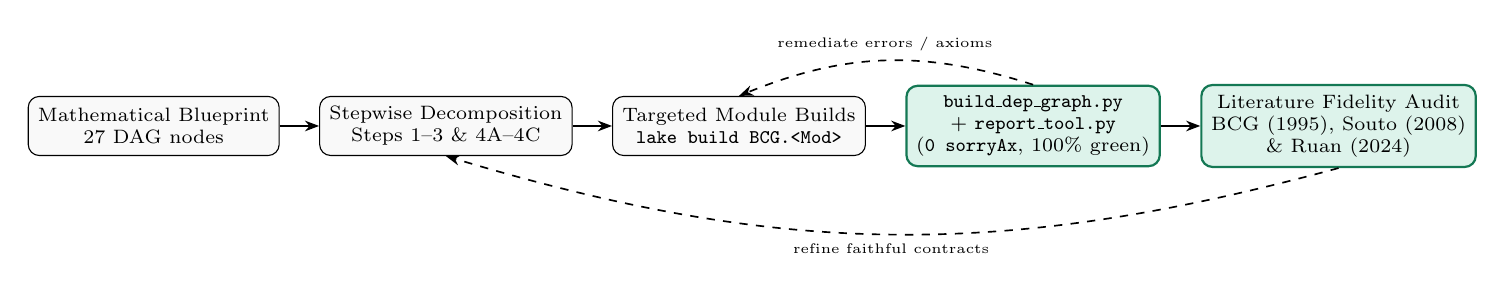
\begin{tikzpicture}[node distance=4.5mm and 5.0mm, every node/.style={font=\scriptsize},
  box/.style={draw,rounded corners,align=center,inner sep=3.5pt,minimum height=7.5mm,fill=gray!5},
  gate/.style={draw,rounded corners,align=center,inner sep=3.5pt,minimum height=7.5mm,fill=bpgreen!15,
               draw=bpgreen!70!black,thick},
  arr/.style={-{Stealth[length=1.8mm]},semithick}]
\node[box] (bp) {Mathematical Blueprint\\\NTotalNodes{} DAG nodes};
\node[box,right=of bp] (orch) {Stepwise Decomposition\\Steps 1--3 \& 4A--4C};
\node[box,right=of orch] (sub) {Targeted Module Builds\\\code{lake build BCG.<Mod>}};
\node[gate,right=of sub] (ver) {\code{build\_dep\_graph.py}\\+ \code{report\_tool.py}\\(\code{0 sorryAx}, 100\% green)};
\node[gate,right=of ver] (san) {Literature Fidelity Audit\\BCG (1995), Souto (2008)\\\& Ruan (2024)};
\draw[arr] (bp)--(orch);
\draw[arr] (orch)--(sub);
\draw[arr] (sub)--(ver);
\draw[arr] (ver)--(san);
\draw[arr,dashed] (ver.north) to[bend right=20] node[above,font=\tiny]{remediate errors / axioms} (sub.north);
\draw[arr,dashed] (san.south) to[bend left=16] node[below,font=\tiny]{refine faithful contracts} (orch.south);
\end{tikzpicture}%
}
\caption{The Lean~4 + \code{leanblueprint} autoformalization and verification pipeline.}
\label{fig:pipeline}
\end{figure}

\paragraph{1. Stepwise Blueprint-First Engineering.}
The formalization proceeded in six self-contained stages: Foundations (spectral trace-det AM--GM,
Souto's bilinear Cauchy--Schwarz, volume entropy), Step~1 (explicit Lorentzian hyperboloid barycenter and
$\Gamma$-equivariance), Step~2 (metric gauge $\Phi_p$ and Fr\'echet derivative of the natural map),
Step~3 (Euclidean change-of-variables and spectral/measure-theoretic equality rigidity), Step~4A (general
rank-one Busemann Hessian and Riccati identity), Step~4B (Minkowski--Ky Fan log-concavity and associative
$\Kfield$-structures), and Step~4C (Ruan's 2024 repair for $\Oct\Hyp^2$). Every theorem and definition is
linked in \code{blueprint/src/content.tex} via \verb|\lean{...}| to \NLeanDecls{} Lean~4 declarations.

\paragraph{2. Two-Tier Verification: Kernel Soundness and Literature Fidelity.}
Every step was verified both syntactically---via \code{lake build}, \code{build\_dep\_graph.py full
-{}-require-all-green}, and \code{report\_tool.py metrics} confirming \code{0 sorryAx} across all
\NLeanDecls{} declarations---and semantically against the original papers \cite{BCG95,Sou08,Rua24},
ensuring that the failure of global property $\mathrm{(P2)}$ on $\Oct\Hyp^2$ and Ruan's line-dependent
replacement $\mathrm{(P2')}$ are faithfully represented.

\begin{thebibliography}{99}\footnotesize\sloppy
\setlength{\itemsep}{1pt}
\bibitem{BCG95} G.~Besson, G.~Courtois, S.~Gallot, Entropies et rigidit\'es des espaces localement
  sym\'etriques de courbure strictement n\'egative, \emph{Geom.\ Funct.\ Anal.}\ \textbf{5} (1995), 731--799.
\bibitem{Sou08} J.~Souto, Note on the volume entropy theorem, preprint / lecture notes, 2008.
\bibitem{Rua24} Y.~Ruan, On a technical detail in BCG's barycenter method, \emph{arXiv:2408.13375} (2024).
\bibitem{YangDG} D.~Yang, Formalization of hyperbolic Busemann functions in Lean~4,
  \code{qinz1yang/differential-geometry} (v0.1.5), 2025.
\bibitem{Lean4} L.~de Moura, S.~Ullrich, The Lean~4 theorem prover and programming language,
  \emph{Proc.\ CADE-28}, LNCS \textbf{12699} (2021), 625--635.
\bibitem{mathlib} The mathlib Community, The Lean mathematical library, \emph{Proc.\ CPP 2020}, 367--381.
\bibitem{TaoPFR} T.~Tao, Formalizing the proof of PFR in Lean4 using Blueprint: a short tour, 2023.
\end{thebibliography}

\newpage
\appendix
\section{Blueprint Dependency Graph}\label{app:graph}

\begin{center}
\vspace{0.5em}
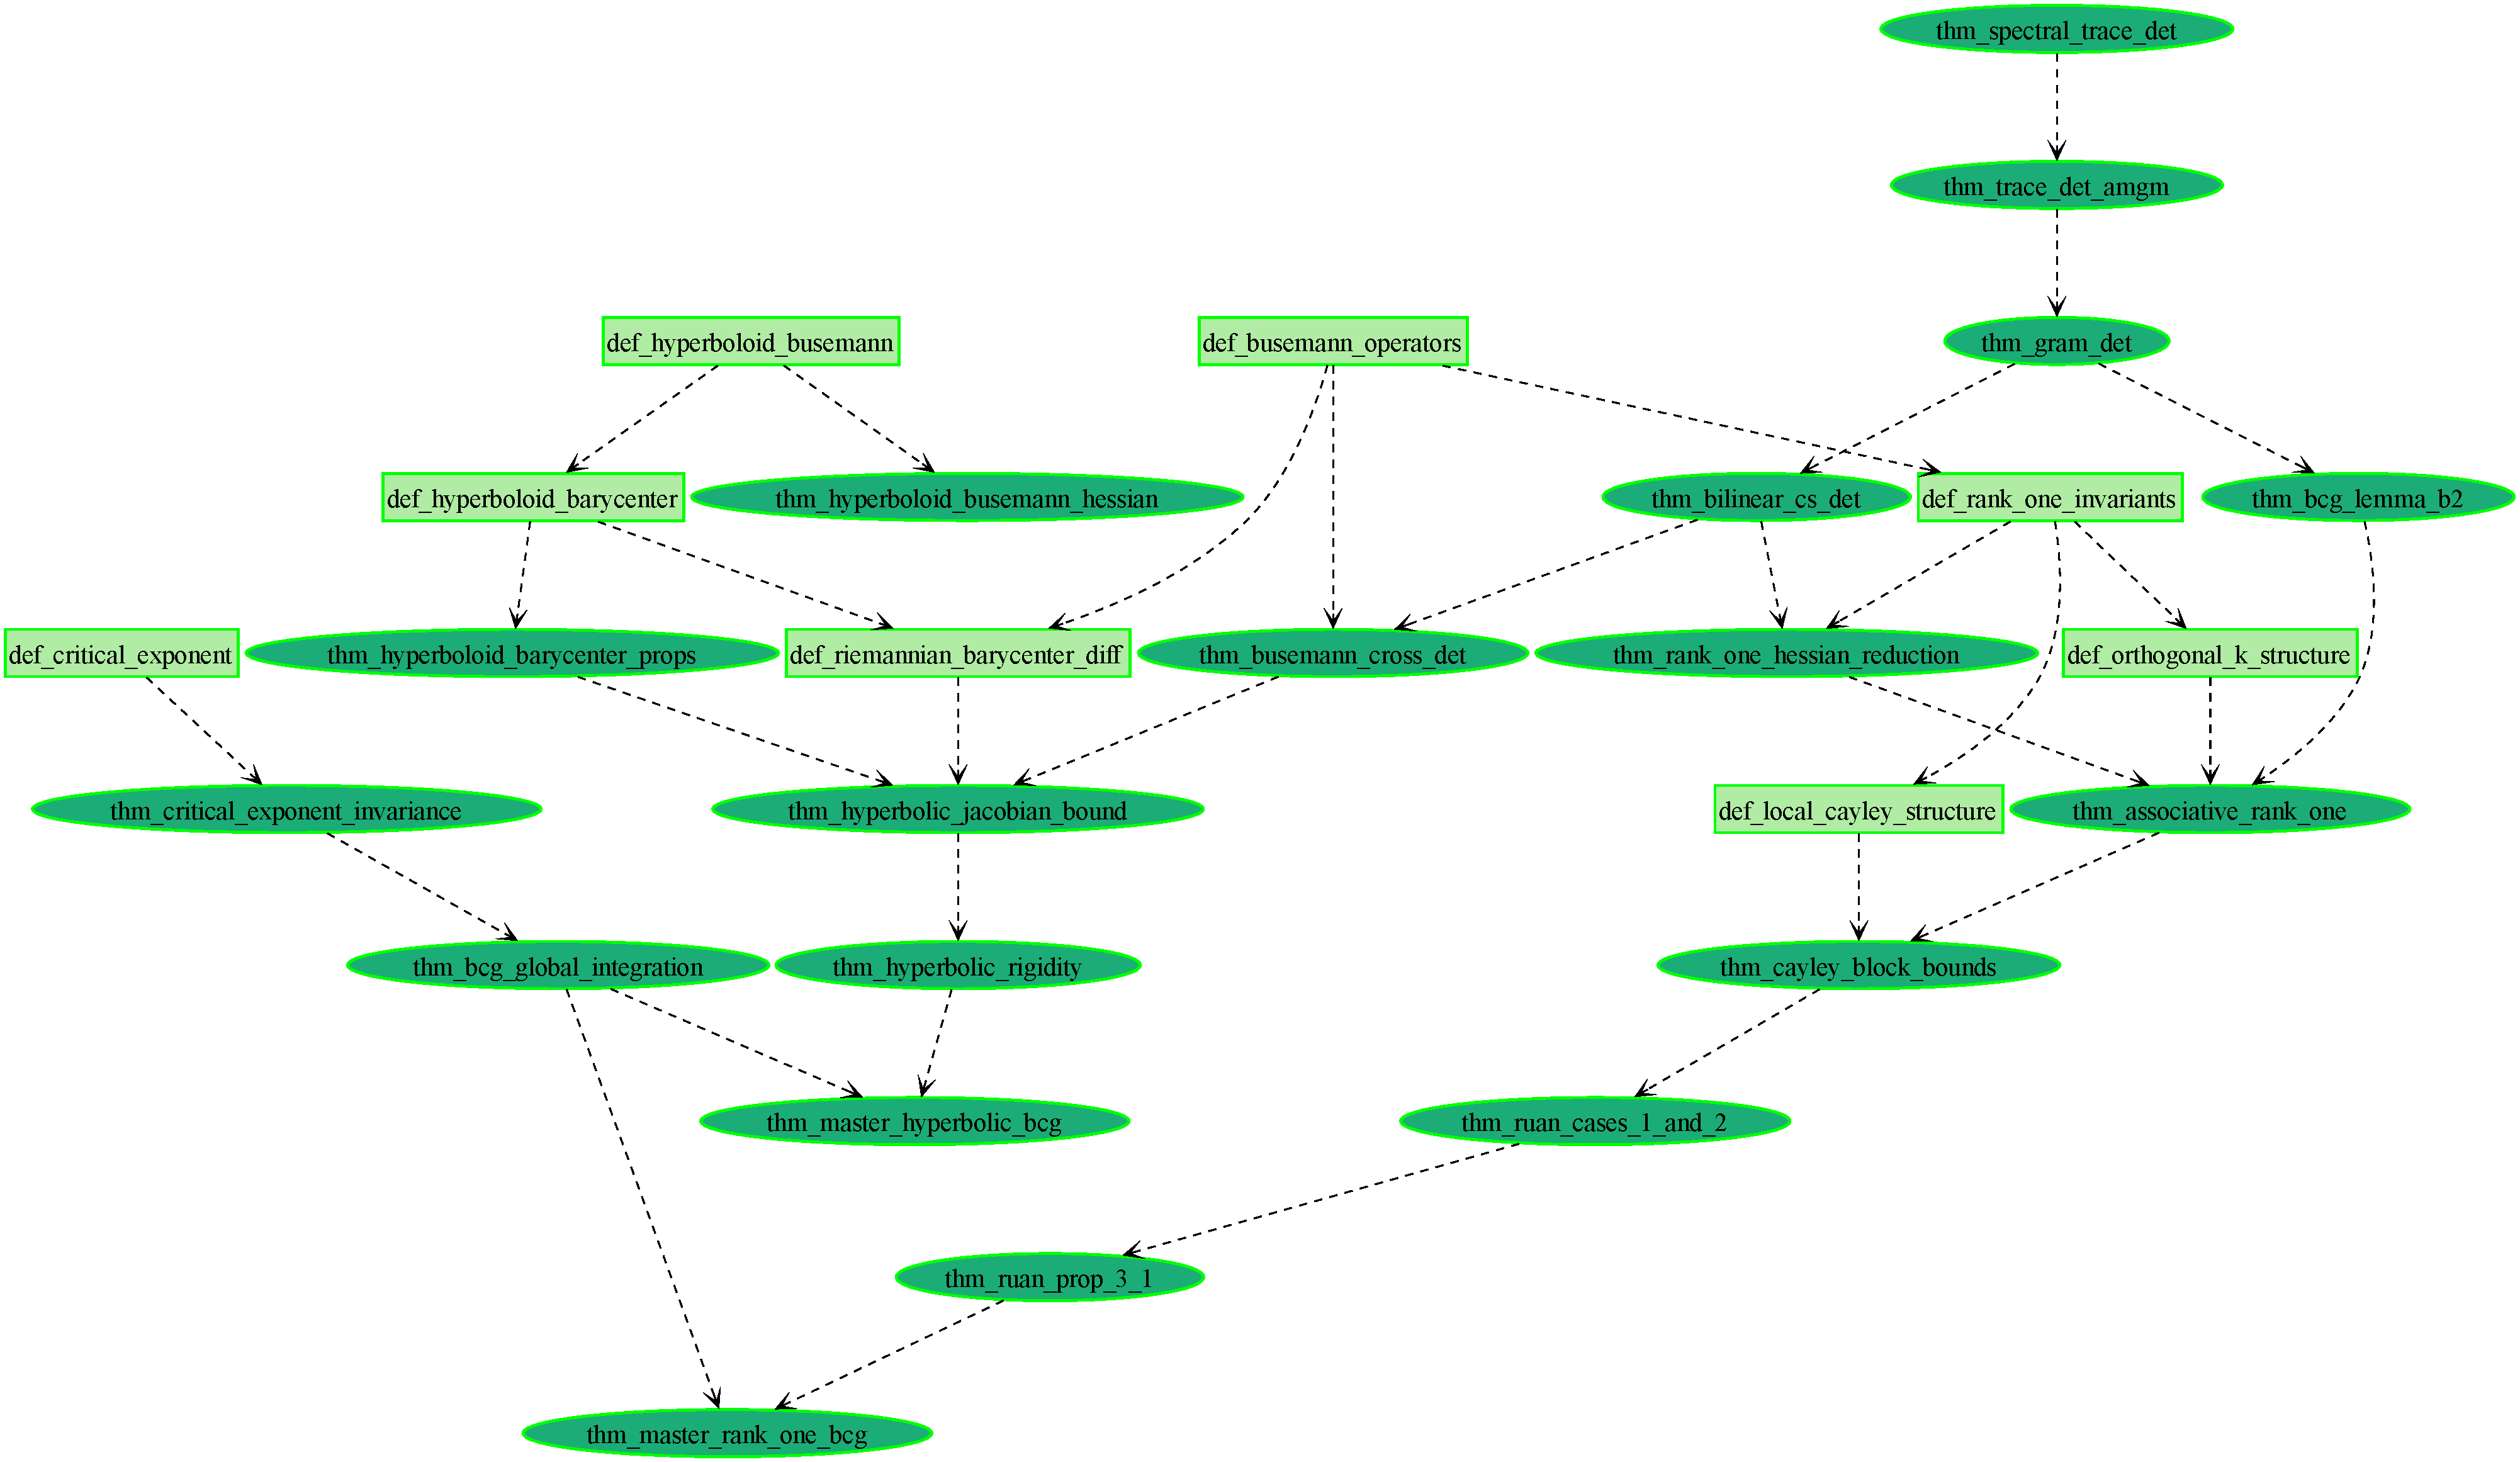
\includegraphics[width=\linewidth,height=0.80\textheight,keepaspectratio]{blueprint_dep_graph.pdf}
\end{center}
\vspace{0.5em}
\noindent\footnotesize\sloppy
\textbf{Figure A.1: Complete \code{leanblueprint} Dependency Graph (Portrait View).}
Generated from \code{blueprint/src/content.tex} via \code{build\_dep\_graph.py}
(interactive HTML version at \code{blueprint/web/dep\_graph\_document.html}).
Arrows point from each foundational definition or lemma to the downstream theorems that depend on it.
\textbf{Node shapes and colors:}
\textbf{Rectangles (\NDefNodes{} nodes, green \code{\#B0ECA3}):} Formalized mathematical definitions.
\textbf{Ellipses (\NProvedNodes{} nodes, dark green \code{\#1CAC78}):} Fully machine-checked theorems,
lemmas, and discharged certificates compiling with \code{0 sorryAx} and standard Lean~4 axioms across
the entire dependency closure.
\textbf{Unproved nodes:} $0$ light green (\code{\#9CEC8B}), $0$ light blue (\code{\#A3D6FF}).\par

\end{document}
